\chapter{Entorno de desarrollo \textit{MIPS32}}\label{ch:entorno-de-desarrollo-mips32}

El desarrollo de \textit{JAMS} está dividido en dos secciones:
la aplicación base y el entorno de desarrollo \textit{MIPS32}.
\textit{JAMS} da soporte al lenguaje ensamblador \textit{MIPS32}
creando una \textbf{capa sobre la aplicación base},
aprovechando todas las herramientas y características explicadas anteriormente.
En este capítulo se abordarán las capacidades de este entorno,
documentando el ensamblador, el simulador y el editor junto
con sus componentes esenciales.


\section{Editor de código \textit{MIPS32}}\label{sec:editor-de-codigo-mips32}

\textit{JAMS} aprovecha la tecnología creada en el entorno base
para el editor de código \textit{MIPS32}.
Este editor es complementado por diferentes nodos presentes en la
aplicación.

Cuando el usuario abre un proyecto y desea editar su código,
debe seleccionar el archivo que desea modificar.
Esto se consigue gracias a la herramienta \textbf{explorador}\ref{fig:jams-explorer-text-hover}, la cual
muestra una representación en forma de árbol de la estructura del proyecto.
El usuario puede expandir y contraer carpetas, así como crear, borrar y
mover archivos.
Si el usuario usa el doble clic sobre un archivo editable, este se abrirá
en el editor.

\begin{figure}[h]
    \centering
    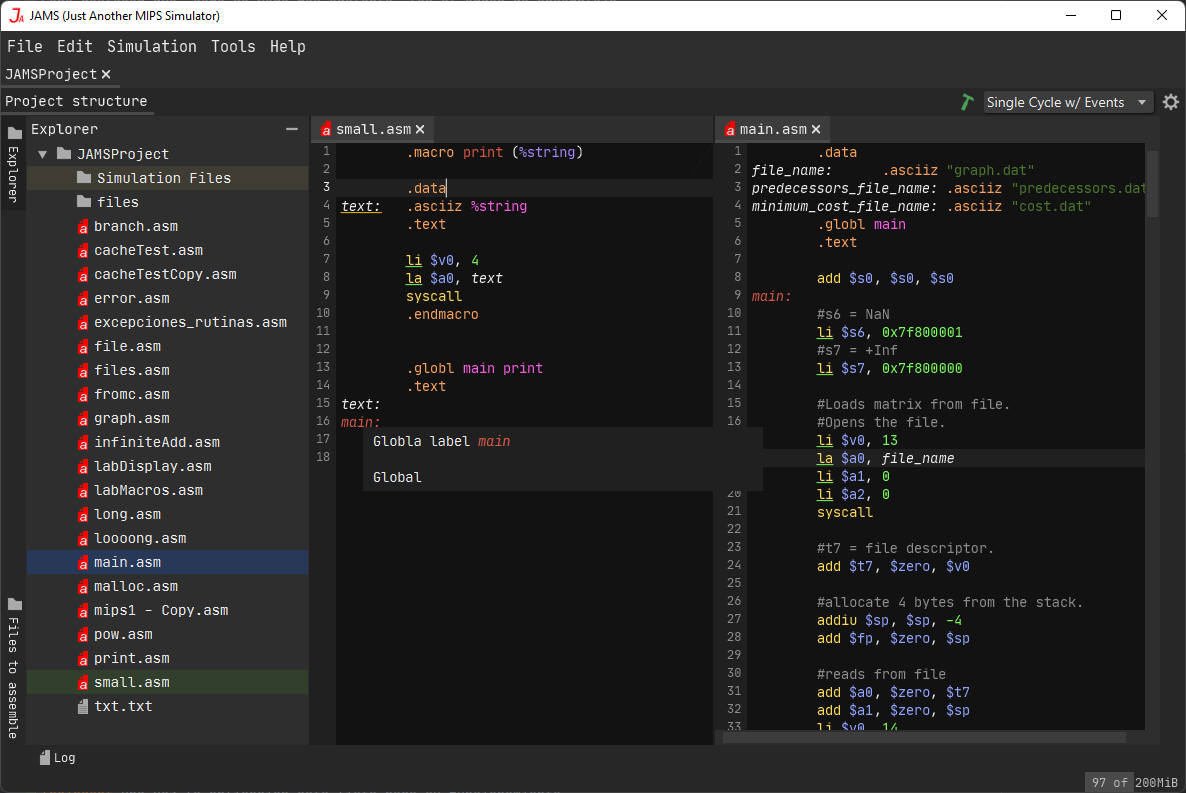
\includegraphics[width=0.8\textwidth]{images/mips/jams-text-hover}
    \caption{Explorador e información sobre un elemento del editor}
    \label{fig:jams-explorer-text-hover}
\end{figure}


El explorador presenta un menú contextual donde el usuario
puede ejecutar varias acciones sobre las carpetas y los archivos
del proyecto.
Una de las opciones más particulares es la opción de añadir o eliminar
archivos de código al ensamblador.
Al ser \textit{JAMS} un entorno de desarrollo basado en \textbf{proyectos},
se ha de proporcionar una manera de incluir o excluir archivos de
la aplicación resultante.
Con este simple sistema, el usuario podrá elegir qué archivos se debe ensamblar.
Los archivos a ensamblar estarán marcados en \textbf{verde} en el explorador,
y aparecerán en orden en el nodo \textbf{\delODR{A}\newODR{a}rchivos a ensamblar}.
Cabe destacar que, como se verá más adelante, \delODR{los} el orden de ensamblaje
\delODR{importa}\newODR{es importante}, por lo que esta herramienta
permite ordenar\delODR{los} de una manera sencilla\newODR{ dichos
  archivos}.

Una vez el usuario haya abierto el archivo a editar, todo su código
aparecerá en la herramienta principal de la sección: \textbf{el visualizador
de archivos}.
Esta herramienta permite mostrar diferentes editores dependiendo del tipo
de archivo abierto.
En la versión sin componentes de \textbf{JAMS}, el editor permite visualizar
imágenes y editar archivos de texto.
En el caso de estos últimos \delODR{archivos}, solo los archivos ensamblador presentan
ayudas, como pueden ser el autocompletador, en resaltador o la documentación.

El visualizador de archivos puede tener varios archivos abiertos
al mismo tiempo.
Cada archivo estará representado por una pestaña que podrá cerrarse.
El usuario podrá arrastrar una de las pestañas a un lado del visualizador
para mostrar dos o más editores al mismo tiempo.

El editor de código \textit{MIPS32} puede considerarse un editor
de texto \textbf{inteligente}: gracias a las librerías creadas en la sección
anterior, es capaz de convertir el texto puro en los diferentes componentes
ensamblador que representa.
El editor también tiene conocimiento de las referencias y el alcance de
todas las etiquetas y macros, tanto en el propio archivo a editar
como en el resto de archivos a ensamblar.
Toda esta información puede ser visualizada por el usuario manteniendo
durante un segundo el ratón encima de un elemento, como se puede observar
en la figura \ref{fig:jams-explorer-text-hover}.

Una vez la aplicación\note{Óscar: ``aplicación'' es un término que
  aparece aquí de la nada, pero al que tú te refieres como si ya
  hubieras hablado de ello. Aquí hay algo que explicar mejor} esté lista para su funcionamiento,
el usuario deberá \textbf{crear una configuración} con todos los parámetros
del ensamblador y del simulador deseados para ejecutar la aplicación.
Esto se consigue pulsando el botón \textbf{configuración} en la parte
superior derecha de la aplicación.
En este menú, el usuario podrá seleccionar el tipo de arquitectura,
el tipo de memoria, las llamadas a sistema que se desean usar,
\newODR{o} el número y tipos de caché que se desean utilizar, entre otras
muchas opciones, como se puede observar en la figura \ref{fig:jams-configuration}.

\begin{figure}[h]
    \centering
    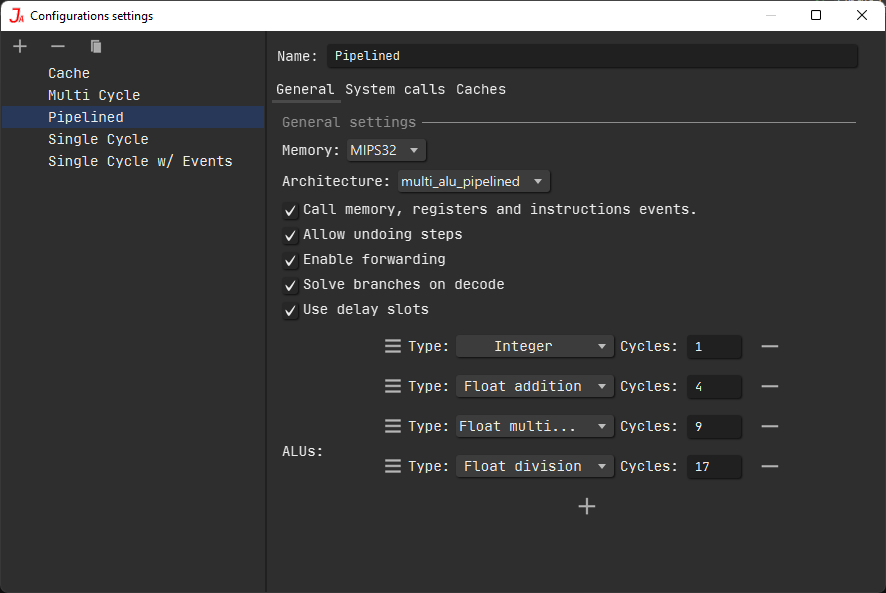
\includegraphics[width=0.8\textwidth]{images/mips/mips-configuration}
    \caption{Configuración de la ejecución de un proyecto}
    \label{fig:jams-configuration}
\end{figure}

Esta configuración será utilizable únicamente en el proyecto
donde se ha creado, y el usuario podrá crear por cada proyecto
un número indeterminado de ellas.
De esta manera, el usuario podrá probar su aplicación en una infinidad
de configuraciones diferentes sin tener que generar un proyecto por cada
configuración.
El usuario podrá seleccionar la configuración que desea ejecutar en
el menú desplegable inmediatamente a la izquierda del botón de configuración.

Finalmente, el usuario podrá llamar al ensamblador pulsando el botón
\textbf{construir proyecto}, representado por un martillo verde.
Una vez pulsado, el informe se desplegará y mostrará el resultado del ensamblador.
Si el resultado es positivo y el código se ha ensamblado, una pestaña con
una simulación aparecerá en el proyecto, permitiendo al usuario simular
el código que acaba de ensamblar.
Cabe destacar que un usuario puede tener diferentes simulaciones abiertas
al mismo tiempo, lo cual amplía las posibilidades de uso de la
aplicación.\note{Óscar: ¿Y si el resultado no es positivo?}


\section{Ensamblador \textit{MIPS32}}\label{sec:ensamblador-mips32}

El ensamblador \textit{MIP32} de \textit{JAMS} es un ensamblador avanzado
usado para ensamblar proyectos \textit{MIPS32}.
Este ensamblador soporta características avanzadas empleadas
comúnmente al programar en ensamblador, como las macros,
las etiquetas globales o las referencias relativas.
El ensamblador ensambla el código de un proyecto en \textbf{cuatro pasos}:
descubrimiento, expansión, asignación de direcciones y asignación de valores.
Se utilizará el siguiente programa para comentar los diferentes pasos del ensamblador:

\begin{lstlisting}[frame=single,label={lst:example.asm}]
    .macro print ( %string )
    .data
text:   .asciiz %string
    .text
    la $a0, text
    li $v0, 4
    syscall
    .endmacro

    .macro printJams ()
    print ("Welcome to JAMS!\n")
    .endmacro

    .text
    .globl main print
main:
local:
    printJams ()
\end{lstlisting}

\subsection{Descubrimiento}\label{subsec:descubrimiento}

En este paso el texto del proyecto se \textbf{descompone en sus primitivas},
permitiendo al ensamblador entender los diferentes componentes de cada línea.
Al final de este paso, las etiquetas globales y las etiquetas del archivo
(etiquetas no definidas dentro de una macro) \textbf{son registradas sin
ningún valor asignado}.
Las macros de cada archivo también son registradas.
El identificador de una macro es definido por su nombre concatena\newODR{n}do
un carácter $-$ al número de parámetros que necesitan.
Este procedimiento se realiza para dar soporte a la sobrecarga de macros.
En el caso de la macro $print$, su identificador sería $print-1$.

\begin{lstlisting}[frame=single,label={lst:descubrimiento}]
Etiquetas globales:
main - XXXXXXXX

Etiquetas del archivo:
local - XXXXXXXX

Macros globales:
print-1

Macros del archivo:
printJams-0
\end{lstlisting}

\subsection{Expansión}\label{subsec:expansion}

En este paso, las llamadas a macros son invocadas,
insertando el código de la macro en la posición de la llamada.
Este código efectúa el primer paso del ensamblador mientras es añadido.
Al ser insertado justo después de la llamada, el código de la macro
también será expandido.

\begin{lstlisting}[frame=single,label={lst:expansion}]
main:
local:
    # Macro printJams-0
    # Macro print-1
    .data # Data returns the previous address.
text:   .asciiz "Welcome to JAMS!\n"
    .text
    la $s0, text
    li $v0, 4
    syscall
    # Endmacro print-1
    # Endmacro printJams-0
\end{lstlisting}

\subsubsection{Alcance}\label{subsubsec:alcance}

Las etiquetas y macros que están dentro de una macro
\textbf{tienen un alcance diferente al del archivo}.
Si la macro es global, el alcance es considerado hijo del alcance global
y no podrá acceder a las etiquetas del archivo que lo invoca.
Si la macro es local, el alcance es considerado hijo del alcance del archivo.

Cuando un alcance es hijo de otro alcance,
\textbf{el hijo podrá acceder a las etiquetas y macros de su padre}.
El hijo también podrá definir nuevas etiquetas y macros con el mismo
identificador que una etiqueta o macro de su padre.
Aunque este comportamiento está permitido, \textbf{el hijo solo podrá acceder
al elemento que él define}.
Esta funcionalidad es llamada \textbf{ocultamiento o \textit{shadowing}}.

\subsection{Asignación de direcciones}\label{subsec:asignacion-de-direcciones}

Una vez el ensamblador haya expandido las macros,
se asignan las direcciones de todas las instrucciones,
etiquetas y directivas que requieran dirección.
Estas direcciones se asignan de manera secuencial.
Existen directivas que pueden modificar el flujo de la asignación,
como es el caso de la directiva $.text$.

\begin{lstlisting}[frame=single,label={lst:address-assignation}]
main:
local:
                    # Macro printJams-0
                    # Macro print-1

0x00400000          .data # Data returns the previous address.
0x10010000      text:    .asciiz "Welcome to JAMS!\n"
0x10010010          .text

                    # la is a pseudo-instruction and
                    # it will be split in two instructions
0x00400000          la $s0, text
0x00400008          li $v0, 4
0x0040000c          syscall

                    # Endmacro print-1
                    # Endmacro printJams-0
\end{lstlisting}

\subsection{Asignación de valores}\label{subsec:asignacion-de-valores}

Como paso final, el ensamblador insertará en memoria los valores
que representan las directivas e instrucciones.

\begin{lstlisting}[frame=single,label={lst:value-assignation}]
                    # Macro printJams-0
                    # Macro print-1

0x10010000          Welcome to JAMS!\n\0
0x00400000          0x3c011001 # la $a0, text
0x00400004          0x34240000
0x00400008          0x24020004 # li $v0, 4
0x0040000c          0x0000000c # syscall

                    # Endmacro print-1
                    # Endmacro printJams-0
\end{lstlisting}

\subsection{Características avanzadas}\label{subsec:características-avanzadas}

El ensamblador permite el uso de técnicas avanzadas en
el desarrollo de aplicaciones en lenguaje ensamblador.

\subsubsection{Referencias relativas}\label{subsubsec:referencias-relativas}

Una directiva o instrucción puede \textbf{referenciar a una etiqueta de manera
relativa} con las referencias especiales $+$ y $-$.
La referencia $+$ hace referencia a la etiqueta siguiente.
La referencia $-$ hace referencia a la etiqueta anterior.
Las referencias relativas \textbf{solo pueden hacer referencia
a etiquetas del mismo alcance}.
No pueden hacer referencia a etiquetas de un alcance mayor.

\begin{lstlisting}[frame=single,label={lst:relative-reference}]
main:
    li $s0, 0
    li $s1, 10
loop:
    printJams ()
    addi $s0, $s0, 1
    bne $s0, $s1, -
\end{lstlisting}

\subsubsection{Macros anidadas}\label{subsubsec:macros-anidadas}

Una macro puede ser definida dentro de otra macro.
Esto es conocido como una \textbf{macro anidada}.
Esta macro solo podrá ser accedida en el alcance de la macro
en la que está declarada.

\begin{lstlisting}[frame=single,label={lst:nested-macro}]
    .macro printJams ()
    .macro print (%string)
    .data
text:   .asciiz %string
    .text
    la $a0, text
    li $v0, 4
    syscall

    .endmacro
    print ("Welcome to JAMS!\n")
    .endmacro
\end{lstlisting}

\subsection{Detalles finales}\label{subsec:detalles-finales}

Como detalle final, cabe destacar que este ensamblador es totalmente personalizable.
Los componentes pueden añadir, eliminar y modificar las instrucciones y directivas
que el ensamblador usa.
La adición de directivas por parte de los componentes permite
\textbf{modificar el comportamiento} del ensamblador, añadiendo
nuevas funcionalidades a este.

Añadir una instrucción o una directiva es muy sencillo en \textit{JAMS}:
un componente únicamente debe añadir una nueva instrucción o
una nueva directiva (representadas por clases) a un conjunto de
instrucciones o directivas ya existente, o crear ese conjunto y registrarlo
con la \textit{API} de \textit{JAMS}.
A este nuevo elemento se le puede añadir un nombre traducible y documentación
a través de un paquete de idiomas.

\note{Óscar: yo quitaría esto}El ensamblador para el \textbf{procesador 6502} utilizado en el
componente creado para el Trabajo de Fin de Grado del Grado en Diseño
y Desarrollo de Videojuegos utiliza una arquitectura muy similar a la mostrada,
teniendo únicamente diferencias en el tratamiento de referencias.

\section{Simulador}\label{sec:simulador}

Un simulador es una pieza de \textit{software} que imita el comportamiento
de un dispositivo.
\textit{JAMS} implementa diversos simuladores para las diferentes
arquitecturas \textit{MIPS32}.
En \textit{JAMS} toma mucho más peso e\delODR{n}\newODR{l} enfoque de la
\textbf{simulación} a nivel de circuito, permitiendo al usuario
conocer el funcionamiento de su aplicación en la arquitectura que desee.
Esto no significa que \textit{JAMS} no optimice la ejecución de código:
todos los componentes están altamente optimizados, pudiendo llegar
la simulación a una velocidad de 40 MHz.

\subsection{Arquitecturas disponibles}\label{subsec:arquitecturas-disponibles}

Actualmente, \textit{JAMS} permite ejecutar el código
en tres arquitecturas \textit{MIPS32} diferentes:
\begin{itemize}
    \item \textbf{Uniciclo}: es la arquitectura más sencilla y
    mejor optimizada.
    Ha sido creada con la velocidad en mente, optando por una
    política de \textbf{cero liberación de memoria}: se crean los mínimos
    objetos posibles, y estos no se liberarán de la memoria hasta que
    la simulación haya terminado.
    Esta política evita que el recolector de basura interfiera en la
    ejecución del simulador, aunmentando su velocidad de ejecución.
    \item \textbf{Multiciclo:} simula una arquitectura
    \textit{MIPS32} multiciclo.
    Es mucho más lenta que la arquitectura uniciclo, ya que requiere
    tener muchos más conceptos en cuenta.
    Las implementaciones de las ejecuciones en esta arquitectura
    están pensadas para ser aprovechadas en arquitecturas más
    complejas, definiendo las lecturas y escrituras de sus
    registros y compartiendo una interfaz transparente para los saltos.
    \item \textbf{Segmentada con varias \textit{ALUs}}: simula
    una arquitectura segmentada o \textit{pipelined} donde coexisten varias
    unidades aritmético-lógicas.
    Esta arquitectura aprovecha mucho código de la arquitectura
    multiciclo, y tiende a ser mucho más lenta.
    Los usuarios pueden modificar el número y tipo de las unidades
    aritmético-lógicas, así como el número de ciclos que requiere
    cada una para completar una operación.
\end{itemize}

\subsection{Estructura del simulador}\label{subsec:estructura-del-simulador}

Independientemente de la arquitectura, todas las simulaciones presentan
la misma estructura básica, idéntica en su base al editor.
Al ejecutar una simulación, el usuario encuentra como nodo principal
un \textbf{visualizador de instrucciones}, mostrado en la figura \ref{fig:jams-simulation}.
Esta herramienta permite visualizar todas las instrucciones que se han
ensamblado, junto a su dirección de memoria, su valor en hexadecimal y
su origen.
El orden de estos valores se puede cambiar en la configuración.
El visualizador también informa sobre las \textbf{instrucciones que se van
a ejecutar} en el siguiente ciclo y, si la arquitectura tiene varias
etapas, mostrará qué etapa ejecutará.
Si la aplicación simulada tiene código para el modo \textit{kernel},
este se mostrará en una pestaña aparte.

\begin{figure}[h]
    \centering
    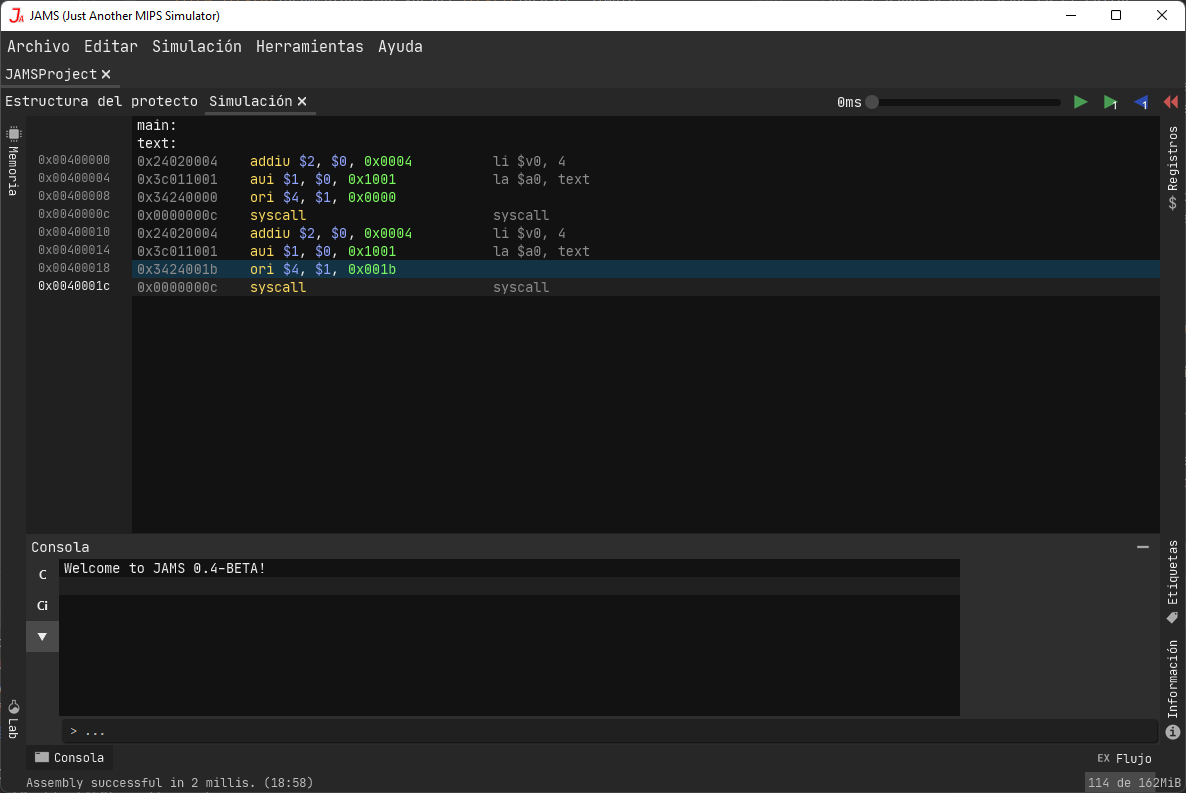
\includegraphics[width=0.8\textwidth]{images/mips/jams-simulation}
    \caption{Interfaz de usuario del simulador}
    \label{fig:jams-simulation}
\end{figure}

En la parte superior derecha se pueden encontrar los
\textbf{botones de control} del simulador.
Estos botones permiten empezar o parar la simulación, ejecutar un
único ciclo, deshacer un ciclo o reiniciar por completo la simulación.
Esta sección también contiene una barra deslizable que permite controlar
la velocidad a la que se ejecuta la simulación.

La ejecución del simulador es totalmente asíncrono, lo cual
impide bloqueos de interfaz cuando una aplicación se está ejecutando.
Todos los componentes y herramientas que desean acceder al simulador
deberán sincronizarse con el hilo del simulador.

El simulador tiene integrad\delODR{o}\newODR{as} \textbf{diversas herramientas} que complementan
el visualizador de instrucciones, permitiendo visualizar y modificar varios
aspectos de la ejecución de un programa.

El nodo más importante es la herramienta de \textbf{memoria},
la cual permite al usuario visualizar y editar el estado de la memoria
\delODR{de la memoria} en el instante actual.
El usuario puede seleccionar el \textbf{modo de representación} de los valores
de la memoria de entre una gran variedad, pudiendo elegir formatos
muy usados como son el formato hexadecimal a formatos específicos
como el \textit{RGB}.
Por último, esta herramienta también permite visualizar el \textbf{estado
de las cachés} del simulador.
Esta información es complementada por la herramienta \textbf{cachés},
la cual informa sobre los fallos y aciertos de las cachés, además de un
informe completo sobre sus acciones.

\begin{figure}[h]
    \centering
    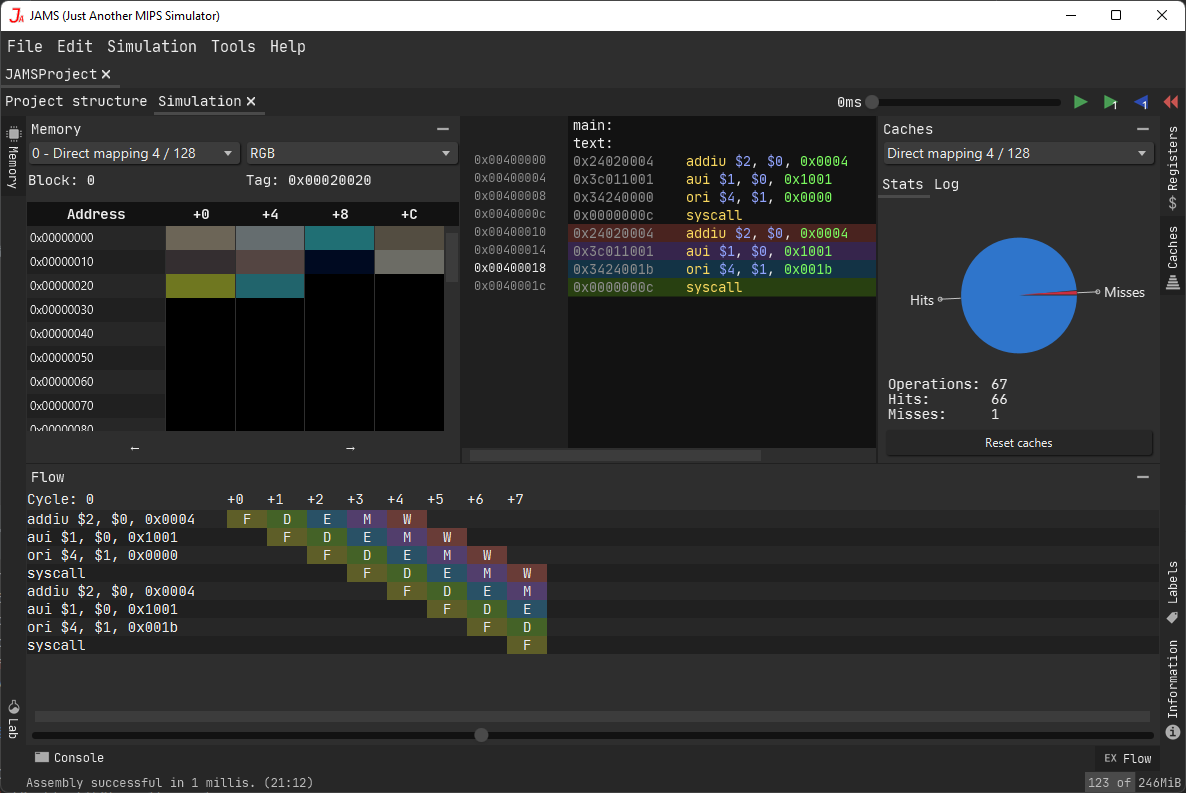
\includegraphics[width=0.8\textwidth]{images/tools/jams-memory-cache-flow}
    \caption{Las herramientas memoria, cachés y flujo en funcionamiento}
    \label{fig:jams-memory-cache-flow}
\end{figure}

Otro nodo muy relevante es la herramienta \textbf{flujo},
la cual registra el estado de todas las instrucciones en cada ciclo
de ejecución.
De esta manera, el usuario podrá saber de un vistazo qué flujo
ha seguido su aplicación en la arquitectura seleccionada.

Como último nodo crucial se encuentra la herramienta
\textbf{laboratorio}, la cual permite al usuario simular
dos visualizadores de siete segmentos, un teclado hexadecimal
y un contador, además de poder generar interrupciones \textit{hardware}
y \textit{software}.

El simulador cuenta con muchos nodos más, como es la
herramienta \textbf{registros}, que permite visualizar y modificar
todos los registros del simulador, la herramienta \textbf{etiquetas},
que guarda las referencias de las etiquetas usadas por el usuario
en el editor, la herramienta \textbf{información}, que muestra
información muy básica y general de la simulación y la
herramienta \textbf{consola}, que permite recibir y enviar
mensajes a la aplicación.

\subsection{Aspectos técnicos}\label{subsec:aspectos-tecnicos}

En esta sección se detallarán brevemente \delODR{algun}\newODR{l}os aspectos técnicos
\newODR{más relevanes} del simulador.

\subsubsection{Memoria}\label{subsubsec:memoria}

La memoria es la parte del simulador y ensamblador
donde se guardan los datos y las instrucciones de una aplicación.
La memoria de la arquitectura \textit{MIPS32} es una memoria de 4 GB
($2^{32}$ bytes) separada en las siguientes secciones:

\begin{figure}[H]
    \centering
    \resizebox{\textwidth}{!}{%
        \begin{tabular}{|l|l|l|l|}
            \hline
            Sección       & Tipo         & Primera dirección & Uso                                                              \\ \hline
            Reserved      & Kernel Level & 0xFFFF0000        & Sección usada para leer y escribir de componentes.               \\ \hline
            Kernel Data   & Kernel Level & 0x90000000        & Datos estáticos del \textit{kernel}.                             \\ \hline
            Kernel text   & Kernel Level & 0x80000000        & Instrucciones del \textit{kernel}.                               \\ \hline
            Stack Segment & User Level   & ↓                 & Pila.                                                            \\ \hline
            Dynamic Data  & User Level   & ↓                 & Memoria reservada en tiempo de ejecución.                        \\ \hline
            Static Data   & User Level   & 0x10000000        & Datos estáticos generados por las directivas al ensamblar.       \\ \hline
            Text Segment  & User Level   & 0x04000000        & Instrucciones del programa.                                      \\ \hline
            Reserved      & Kernel Level & 0x00000000        & Sección usada por el sistema operativo. Sin uso en el simulador. \\ \hline
        \end{tabular}%
    }
    \caption{Estructura de la memoria en \textit{MIPS32}}
    \label{fig:memory-table}
\end{figure}

Reservar 4 GB de memoria para cada simulación no es una buena idea:
ocuparía una gran parte de la RAM de un computador y la gran mayoría no se utilizaría.
Para evitar este problema existen varias técnicas para la
implementación de la memoria:
\begin{itemize}
    \item Limitar la memoria de cada sección.
    Esta técnica es la empleada en el simulador \textit{MARS}.
    \item Partir las secciones en sub-secciones.
\end{itemize}

\textit{JAMS} implementa la segunda opción:
cada sección de memoria es separada en bloques de 4 KB.
Estas secciones no serán reservadas en memoria
hasta que sean necesarias.
Con esta implementación, se reserva un array inicial de
$2^{22}$ ($2^{32}$ / $2^{12}$) entradas, lo que equivaldría
a unos simples 8 MB\@.
Según el uso de la memoria dentro del simulador,
se irán reservando trozos de 4 KB\@.

\subsubsection{Cachés}\label{subsubsec:caches}

Las cachés son memorias más pequeñas y más rápidas que están
situadas entre la memoria y el procesador.
Los computadores actuales suelen tener varios niveles de caché,
actuando unas sobre otras.
En \textit{JAMS}, las memorias funcionan de manera muy similar.
Tanto las cachés como las memorias implementan la interfaz $Memory$.
Esta interfaz define los métodos de lectura y escritura.
Cuando un simulador necesita leer o escribir en la memoria,
llama al método correspondiente en su memoria.
Lo que no sabe el simulador es que su \textbf{memoria puede ser una caché}
con una referencia a otra memoria.
Cuando una caché es invocada en una operación de lectura o escritura,
es ella la que gestiona la operación y,
si es necesario, accede a la memoria que tiene como referencia.
Con esta sencilla arquitectura se genera una jerarquía de memorias
muy similar a la que encontramos en computadores reales.

Actualmente, \textit{JAMS} soporta tres tipos básicos
de cachés: \textbf{cachés por correspondencia directa},
\textbf{cachés asociativas} y \textbf{cachés asociativas por conjuntos}.
Todos los tipos de cachés soportan tanto el modo \textit{write-back}
como el modo \textit{write-through}.

\subsubsection{Interrupciones}\label{subsubsec:interrupciones}

Las interrupciones permiten informar sobre eventos al
simulador.
Cuando una interrupción sucede, el simulador entrará en el
modo \textit{kernel}, saltando automáticamente al controlador
de interrupciones proporcionado por el proyecto.
Si la simulación no tiene implementado ningún controlador de
interrupciones, su ejecución termina de manera abrupta.

\begin{figure}[h]
    \centering
    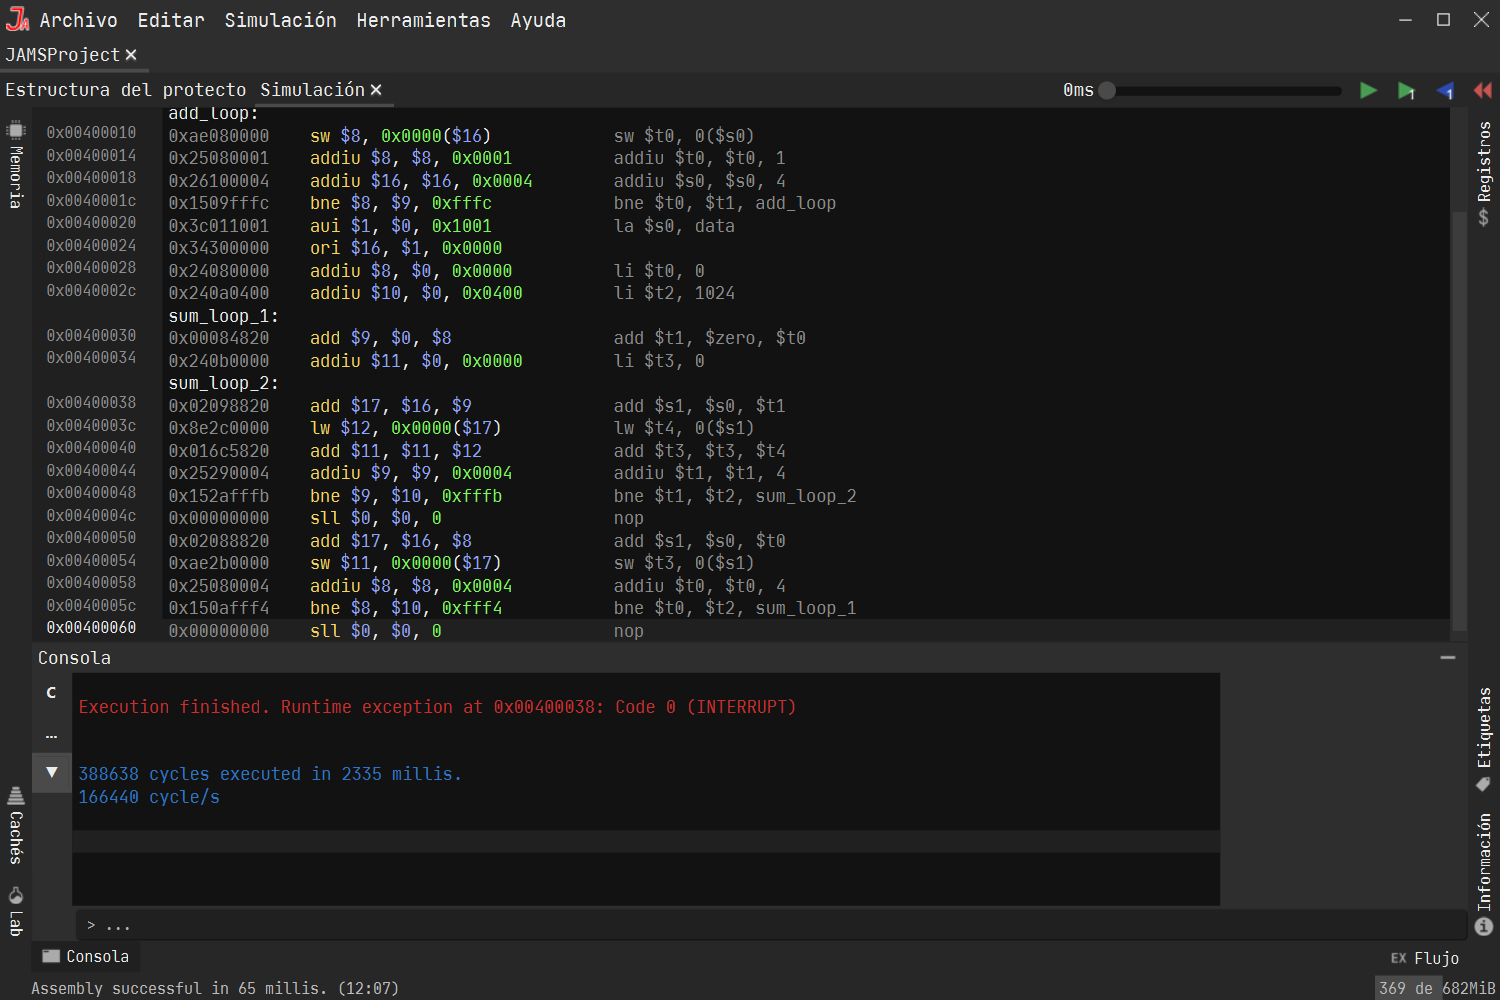
\includegraphics[width=0.8\textwidth]{images/mips/jams-exception}
    \caption{Excepción en una simulación}
    \label{fig:jams-exception}
\end{figure}

Cuando varias interrupciones ocurren al mismo tiempo,
estas se ejecutan de manera secuencial, teniendo más prioridad
la interrupción \textbf{con mayor nivel}.
Si una interrupción ocurre mientras el simulador está en el
modo \textit{kernel}, esta se añade a la cola de interrupciones
y se procesará cuando el simulador pase al modo usuario.

Las interrupciones pueden clasificarse en interrupciones
\textit{software} e interrupciones \textit{hardware}:
\begin{itemize}
    \item \textbf{Interrupciones \textit{software}:} permiten informar
    al programa de errores o excepciones en la simulación.
    Este tipo de interrupciones deben contener una causa que
    el programa puede\note{Óscar: ¿pueda y no puede?} leer.
    Estas interrupciones son de nivel 1.
    \item \textbf{Interrupciones \textit{hardware}:} permiten informar
    al programa de eventos generados por los diferentes componentes
    conectado\newODR{s} al simulador.
    Estas interrupciones están definidas por \delODR{un nivel entre el}
    nivel\newODR{es, definidos del} 2 al 63.
    \delODR{Este nivel permite}\newODR{Estos niveles permiten} calcular la dirección de memoria
    del punto de entrada del controlador de interrupciones.
\end{itemize}

El simulador gestiona las interrupciones usando la
implementación presentada en la figura \ref{fig:mips-exception-generator},
extraída del documento
\textit{MIPS® Architecture For Programmers Vol. III}\cite{MIPS_VOL_3},
permitiendo generar hasta 63 tipos diferentes de excepciones.

\begin{figure}[h]
    \centering
    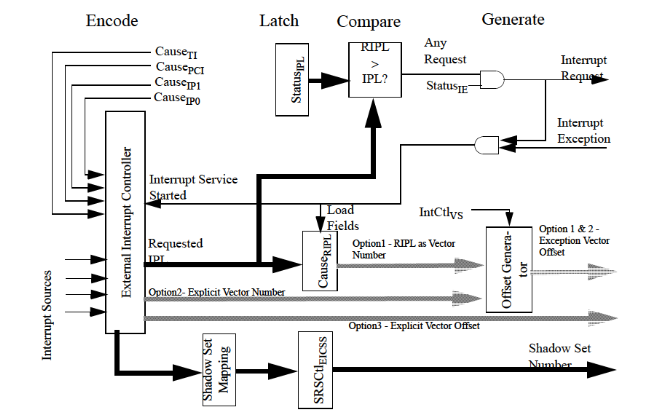
\includegraphics[width=\textwidth]{images/mips/mips-exception-generator}
    \caption{Generador de excepciones para excepciones externas}
    \label{fig:mips-exception-generator}
\end{figure}
